\documentclass[24pt,pdf,hyperref={unicode}]{beamer}
\usepackage[utf8]{inputenc}
\usepackage{aiml}


\begin{document}

\begin{frame}\frametitle{Точное вычисление нечетких операций}
\uncover<+->{}
\uncover<+->{$$
\mu_X(x)=\max\left[0,1-\left(\frac{x-\ceil{X}}{q}\right)^2\right]
$$}
\uncover<+->{$$
\mu_Y(y)=\max\left[0,1-\left(\frac{x-\ceil{Y}}{q}\right)^2\right]
$$}
\uncover<+->{$$
Z=\arctan Y/X
$$}
\uncover<+->{$$
\mu_Z(z)=\max_{x,y\ z=\arctan(y/x)}\mu_X(x)\mu_Y(y)
$$}
\uncover<+->{$$
z=\arctan(y/x)\Rightarrow y=x \tan z
$$}
\uncover<+->{$$
\mu_C(z)=\max_{x\in\mathbb{X}}\left(1-(px-q)^2\right)\left(1-(rx-s)^2\right)
$$}
\end{frame}

\begin{frame}\frametitle{Точное вычисление нечетких операций}
$$
\mu_C(z)=\max_{x\in\mathbb{X}}\left(1-(px-q)^2\right)\left(1-(rx-s)^2\right)
$$
\only<2>{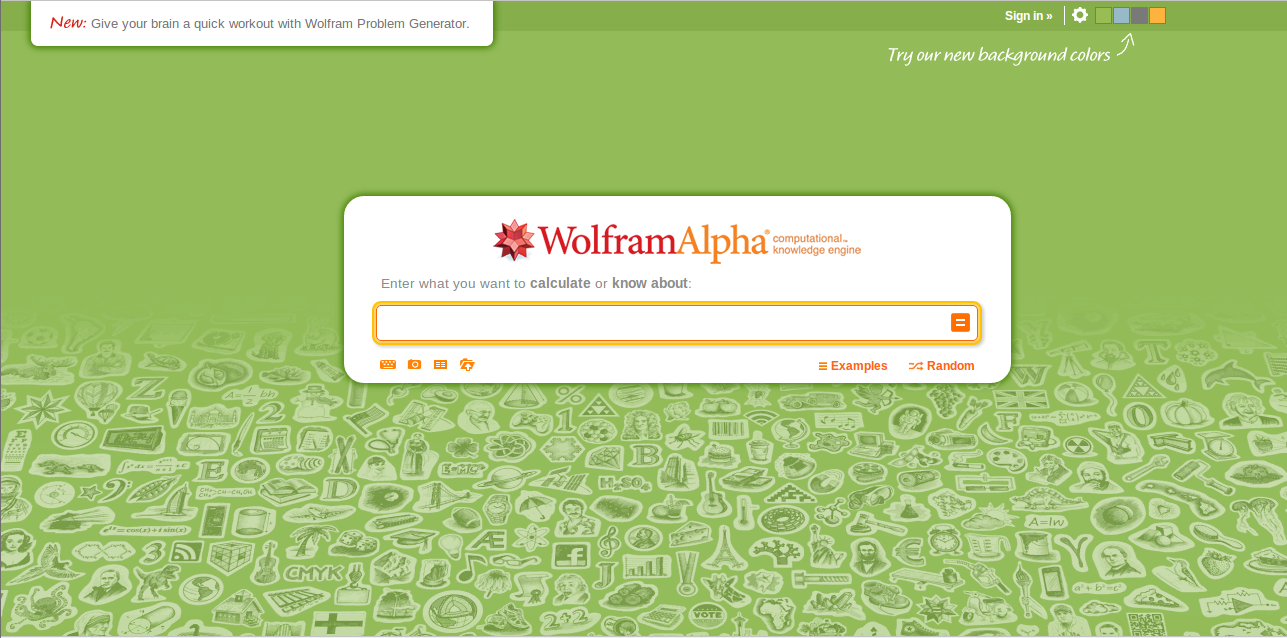
\includegraphics[width=\textwidth]{wolfram.png}}
\only<3>{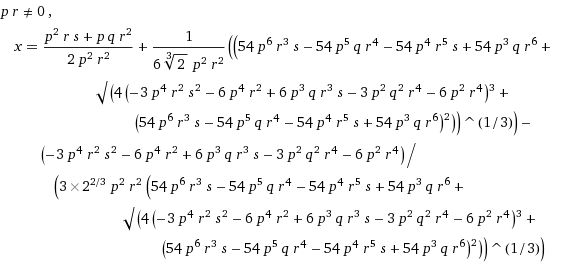
\includegraphics[width=\textwidth]{roots.png}}

\end{frame}


\end{document}